\section{Architecture}\label{sec:architecture}

\textbf{Authoriship: } Written by Oliver Bruski\\

\vspace*{4mm}


The challenge of software architecture is to create a structured
solution that meets all given requirements and constraints for a domain
problem. It presents an abstract structure on the system and includes
the building blocks of the solution with their interaction without
focusing on the low-level implementation details like interface design
\cite{Garlan&Shaw.1994}. Moreover, the system architecture presents a blueprint
not only for the system but for the project as well. The architecture
can be utilized to divide the development team into groups. The process
of producing a system architecture starts with a high-level view of the
whole project and is incrementally broken down into smaller subsystems
\cite{Bass&Clements&Kazmann.2012}.

In order to design a reasonable architecture, it is necessary to know
the domain of the problem. Think of the domain as the problem area and
the domain model driven design as the solution for this specific
problem. The domain model represents an organized and structured view on
the problem. Consequently, the domain should be defined in the beginning
of a project to avoid misunderstandings and put everyone non the same page. The Domain driven design focuses on
understanding and interpreting the specific aspects of the given
problem.

This chapter will elaborate on the motivation and the decisions we made.
Further, we discuss existing architecture for similar problem
statements. The main part will of this chapter will present the created
architecture and how it evolved over time. Finally, we conclude the
chapter with a critical analysis of the architecture and discuss
possible future improvements.

\subsection{Motivation}\label{motivation}

Due to the distributed nature of the project, the target was to build
upon loosely coupled components. For this purpose, a microservice
architectural design was the best fit. Using a microservice approach
allowed to decouple the system and divide it into independent modules.
Microservices interact through specified interfaces in contrast to a
monolithic system were the different modules depend on each other due to
inheritance of classes for example. By communicating just through
specified interfaces no unintended dependency will be formed. Every
interaction between services has to be implemented explicitly \cite{Wolff.2016}.

A pleasant side effect of the loose coupling of components is that it
allowed to divide the team according to the main building blocks. Each
component was the responsibility of a different group. Furthermore, the
absence of string dependence and inheritance among services allowed to
use several technologies and programming languages. Thus, every group
was able to use the language that suited the purpose best. In addition
to independent development, we were able to conduct tests independent
from other components. This was necessary due to the limited budget for
infrastructure and deployment. Hence, we were able to test every
component stand-alone before testing the whole system.

Another benefit of a microservice approach is that nearly every
component is independently scalable and load-balancing can be
implemented using smart routing. Furthermore, by creating stateless
components, horizontal scalability was easily achievable. By replacing
point-to-point communication with a distributed messaging system between
the different building blocks, we were able to improve scalability even
more and decouple even further. Firstly, the queue introduces a
separation layer between the components, which allows to easily exchange
one component without altering the other one. Furthermore, the queue can
work as a buffer to protect the components from temporary peaks in the
load.

Obviously, there are some challenges that have to be resolved to harness
all the benefits of microservice architecture. In contrast to a
monolithic solution every microservice can be deployed independently.
Also, this is beneficial for our limited budget and allows to test and
deploy the components separately it comes with a price. A complex system
can consist of many microservices that have to be deployed one by one,
thus it is crucial to automate the deployment process. If implemented
correctly, a continuous-delivery-pipeline presents huge benefits not
only for microservices. We adapted the continuous-delivery-pipeline
introduced by Wolff and customized it to fit our workflow.
(Commit -- local test -- system test -- performance test) \cite{Wolff.2016}. It started with a commit onto
GitHub and was followed by local tests. Here again the microservices
approach presented its benefits, since it allowed for independent
testing. Unfortunately, just towards the end of the project we were able
to conduct system tests and examine the functionality in an end-to-end
workflow. Nevertheless, through meticulous local testing and loose
coupling of the components we were able to omit huge changes to the
components when working in ensemble as a whole. Finally, we conducted
performance test for the complete system to ensure high performance and
prove scalability. Besides, the performance of single components was
evaluated to avoid bottlenecks.

In addition to the challenges imposed by the deployment process,
operating a microservice system presents its own set of challenges.
Every component is monitored independently and the logs have to be
gathered in a central storage. Logging is necessary to ensure
availability of each service. Should a service terminate unexpectedly,
the administrator has to restart the service to ensure the performance
of the whole system. Though, the system should be still available during
the downtime of a single service with some possible losses on
functionality. Chapter \ref{sec:infrstructure} will discuss how
we enabled recovery and fault-tolerance of the system.

The next section, will presented the specific requirements for the given
problem statement and how microservice architecture presents a solution
for it.

\subsection{Requirements for the System}\label{requirements-of-the-whole-platform}

To create a system that is able to resolve all the presented objectives,
we identified the following architectural requirements:

\begin{itemize}
\tightlist
\item
  \textbf{Scalability}
\item
  \textbf{Extensibility}
\item
  \textbf{High Performance}
\item
  \textbf{Fault-tolerance}
\end{itemize}

Systems are expected to grow over time and handle increasing load. Thus,
we need a system architecture that allows to scale effortlessly and
benefit from economies of scale. Besides, following the microservice
architecture components should include as little functionality as
necessary and in addition, not share any state to avoid synchronization.
Finally, single-points-of-failure must be avoided to ensure availability
even if a single component fails \cite{Chatzakis.2016}.

Next, hoping that the created system will provide value to the open data
community and more and more people will use it, it is necessary to
handle increasing workloads and ensure high performance even under peak
loads. Additionally, the architecture must be fault-tolerant and ensure
good performance even if some nodes fail obviously, losing some
functionality.

Moreover, the system is expected to be extensible to allow for
contributions by the community. Specifically, we offer an importing
framework in order to simplify sharing your own environmental sensor
data on our platform. Thus, the architecture must be designed in a way
that allows to incorporate modules from other developers without
significant changes to the system.

Finally, the goal of the system is to provide an end-to-end solution for
open data enthusiasts to share their collected data and retrieve it
together with data from other sources and add value to the data through
smart combination. This requirement decomposes into four steps:

\begin{enumerate}
\def\labelenumi{\arabic{enumi}.}
\tightlist
\item
  Collect and ingest data from various heterogeneous sources
\item
  Process and transform the data
\item
  Provide persistend storage for the data
\item
  Offer a uniform interface to retrieve all data contributed
\end{enumerate}

\subsection{Design Decision}\label{design-decision}

This section will discuss the decision concerning the architectural
design on a higher level. decision for specific technologies and
components will be presented in the following chapters. To tackle all of
the mentioned requirements, we decided upon the architecture depicted in figure \ref{fig:architecture_4}.

\begin{figure}
	\centering
		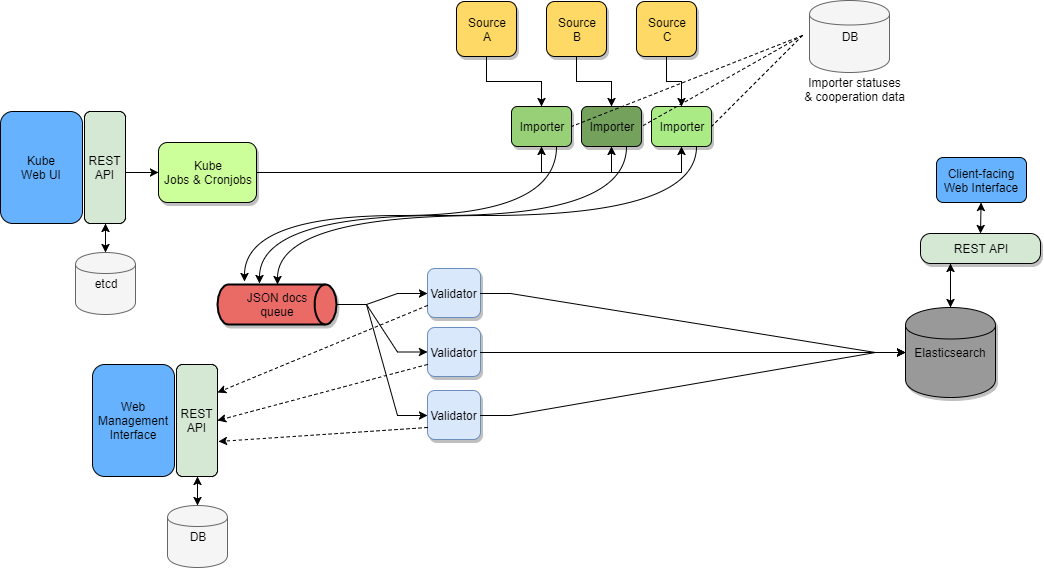
\includegraphics[width=1.00\textwidth]{images/170713_architecture4.png}
	\caption{Final Architecture}
	\label{fig:architecture_4}
\end{figure}

The final architecture is formed from five building blocks:

\begin{itemize}
\tightlist
\item
  Importers
\item
  Consumers
\item
  Database
\item
  Infrastructure Monitoring \& Scheduling
\item
  Data Source Metadata Management
\end{itemize}

The main goal was to create components that are stateless and do not
need to synchronize. This allowed our system to scale horizontally
without additional effort. To omit bottlenecks, we chose components that
are distributed by design. Moreover, as discussed earlier every building
block should be independent from each other. Thus, every building block
could have been developed independently and is easily exchangeable when
necessary. The components communicate through a technology-agnostic
interface or are separated by a distributed messaging system. Now we
will discuss how we designed our building blocks to satisfy the
presented requirements.

\subsubsection{Importers}\label{importers}

The system is supposed to handle all kinds of heterogeneous sources. At
this point we focus on the heterogeneity of the data size and frequency
rather than the different protocols and interfaces. Since most sources
have a unique frequency at which they update their data and the amount
of measurements differs between sources, the system should allow to
schedule the importing task accordingly. Hence, every importer runs as
an independent service with a specific lifecycle (run-time and frequency
of execution) and specific scope (timeframe). Upon finishing its job the
task terminates and the resources are released to allow for maximal
resource utilization. Following a microservice design, every importer
manages its state independently from the system and can restart from a
checkpoint in case of failure. Using such a design allows for decoupled
services that can be spawned independently, are fault-tolerant and
easily scalable by adding a new importer for a different time period or
source.

\subsubsection{Messaging System}\label{messaging-system}

To decouple the components even further we introduced a queuing system
to transport and buffer messages between the importers and consumers.
Since this building block is crucial to ensure scalability and should
protect the system from workload peaks. Following the ``think big''
approach, we imagined a system capable of handling millions of
concurrent requests. In order to achieve such a high throughput, the
system has to be designed in a distributed manner. To additionally
introduce fault-tolerance we need a service that replicates data
automatically to compensate for crashed nodes. Automatic partitioning
would be a further benefit to assist load-balancing. In contrast to a
monolithic application, by decoupling the components with a distributed
messaging system, the autonomous services can be deployed independently
and enable fault-tolerance for the system as a whole.

\subsubsection{Database}\label{database}

When it comes to the choice of a database in addition to the
requirements that applied for the other building blocks the schema of
the data is what is of major concern. The data model and the specific
choice of a database technology will be discussed in more detail in
chapter \ref{sec:database}. At this point the decision for relational or
NoSQL databases has to be made. The designed system is supposed to
interact with many heterogeneous source and data models. Thus, making it
hard to fit into a relational model. Additionally, the emphasis for our
system is availability rather than consistency, which is why we can
spare transactions in order to achieve higher availability and
performance. Most NoSQL databases are designed to partition and shard
the data to increase performance and sacrifice consistency \cite{Chatzakis.2016}.
Moreover, asynchronous replication is good enough in terms of
consistency, when the availability of the system is increased.

Concluding, the choice in favor of a NoSQL solution was the right
decision. NoSQL databases allow for higher flexibility and are designed
to scale across several nodes.

\subsection{Existing solutions}\label{existing-solutions}

It is always advisable to research existing solutions and contributions to the given problem. By doing so, first, one avoids doing the same work again and emphasize that the proposed work provides added value. Furthermore, one can learn from existing solutions and approaches to solve the given problem. In this section we will discuss the existing architectures to resolve the challenge of collection huge amounts of data and, process and store it persistently.

Our problem statement is to collect open sensor data, process it in batches, store it persistently and provide it to the user through a unified interface. The Amazon Web Services (AWS) Lab offers an extensive collection of reference architectures for their cloud platform. Nevertheless, it is build on top of the AWS cloud service, most of the offerings by AWS can be replaced by open source solutions with similar functionality in order to run on different infrastructure. We identified three proposed reference architecture that fit our problem statement. Figure \ref{fig:aws-refarch} shows the IoT Reference Architecture and the Stream Processing Reference Architecture on AWS. Even though the shown reference architecture do not mirror our whole pipeline, they overlapp in some aspects, which makes it interessting to investigate them further. The third reference architecture, Batch Processing with ECS, suggests more of an approach to employ containers with AWS' container services. Since we wanted to create a provider independent platform, we did not pursue it any further. Though, we adapted a container approach using docker to abstract away from the underlying infrastructure.

Our use case is comparable to a IoT service. The main difference is that we do not ingest data via stream into our system but rather in batches at scheduled times. Nevertheless, the data arrives in myriad different formats and in addition, depending on the success and popularity of the system, at some point in time the batches will be so frequent that it might resemble a stream. The workflow is similar to the one we wanted to build. The data enters the system, gets processed by a small and simple component and then is stored for querying.

The stream processing architecture is a little simpler. Though, here as well the pipeline is comparable to the workflow that we employ. Besides the low-latency storage in DynamoDB a archival storage in S3 is created. We believe that retrieving histroical data together with new recent data is one aspect that adds value to the retrieved data thus, we serve the data independent of the arrival time in our main storage solution. Nevertheless, it presents a possible solution on how to store data that is not frequently queried when the stored amount is hard to be processed by a single engine.

\begin{figure}%
	\centering
	\subfigure[AWS IoT Reference]{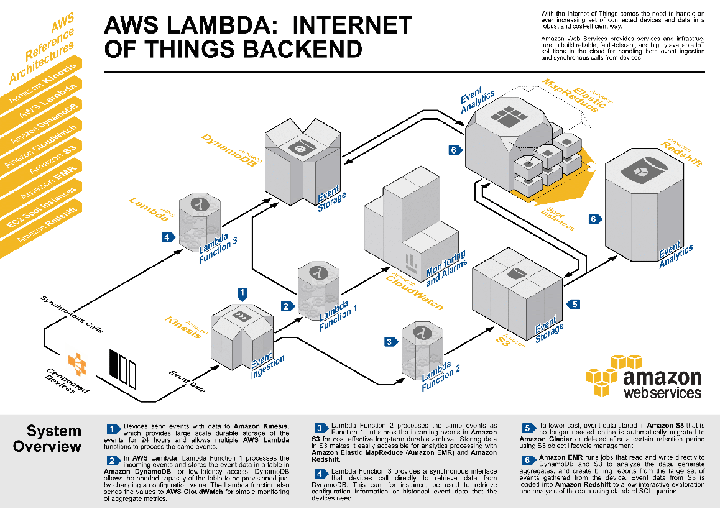
\includegraphics[width=0.45\textwidth]{images/lambda-refarch-iotbackend.png}}
	\subfigure[AWS Stream Processing Reference]{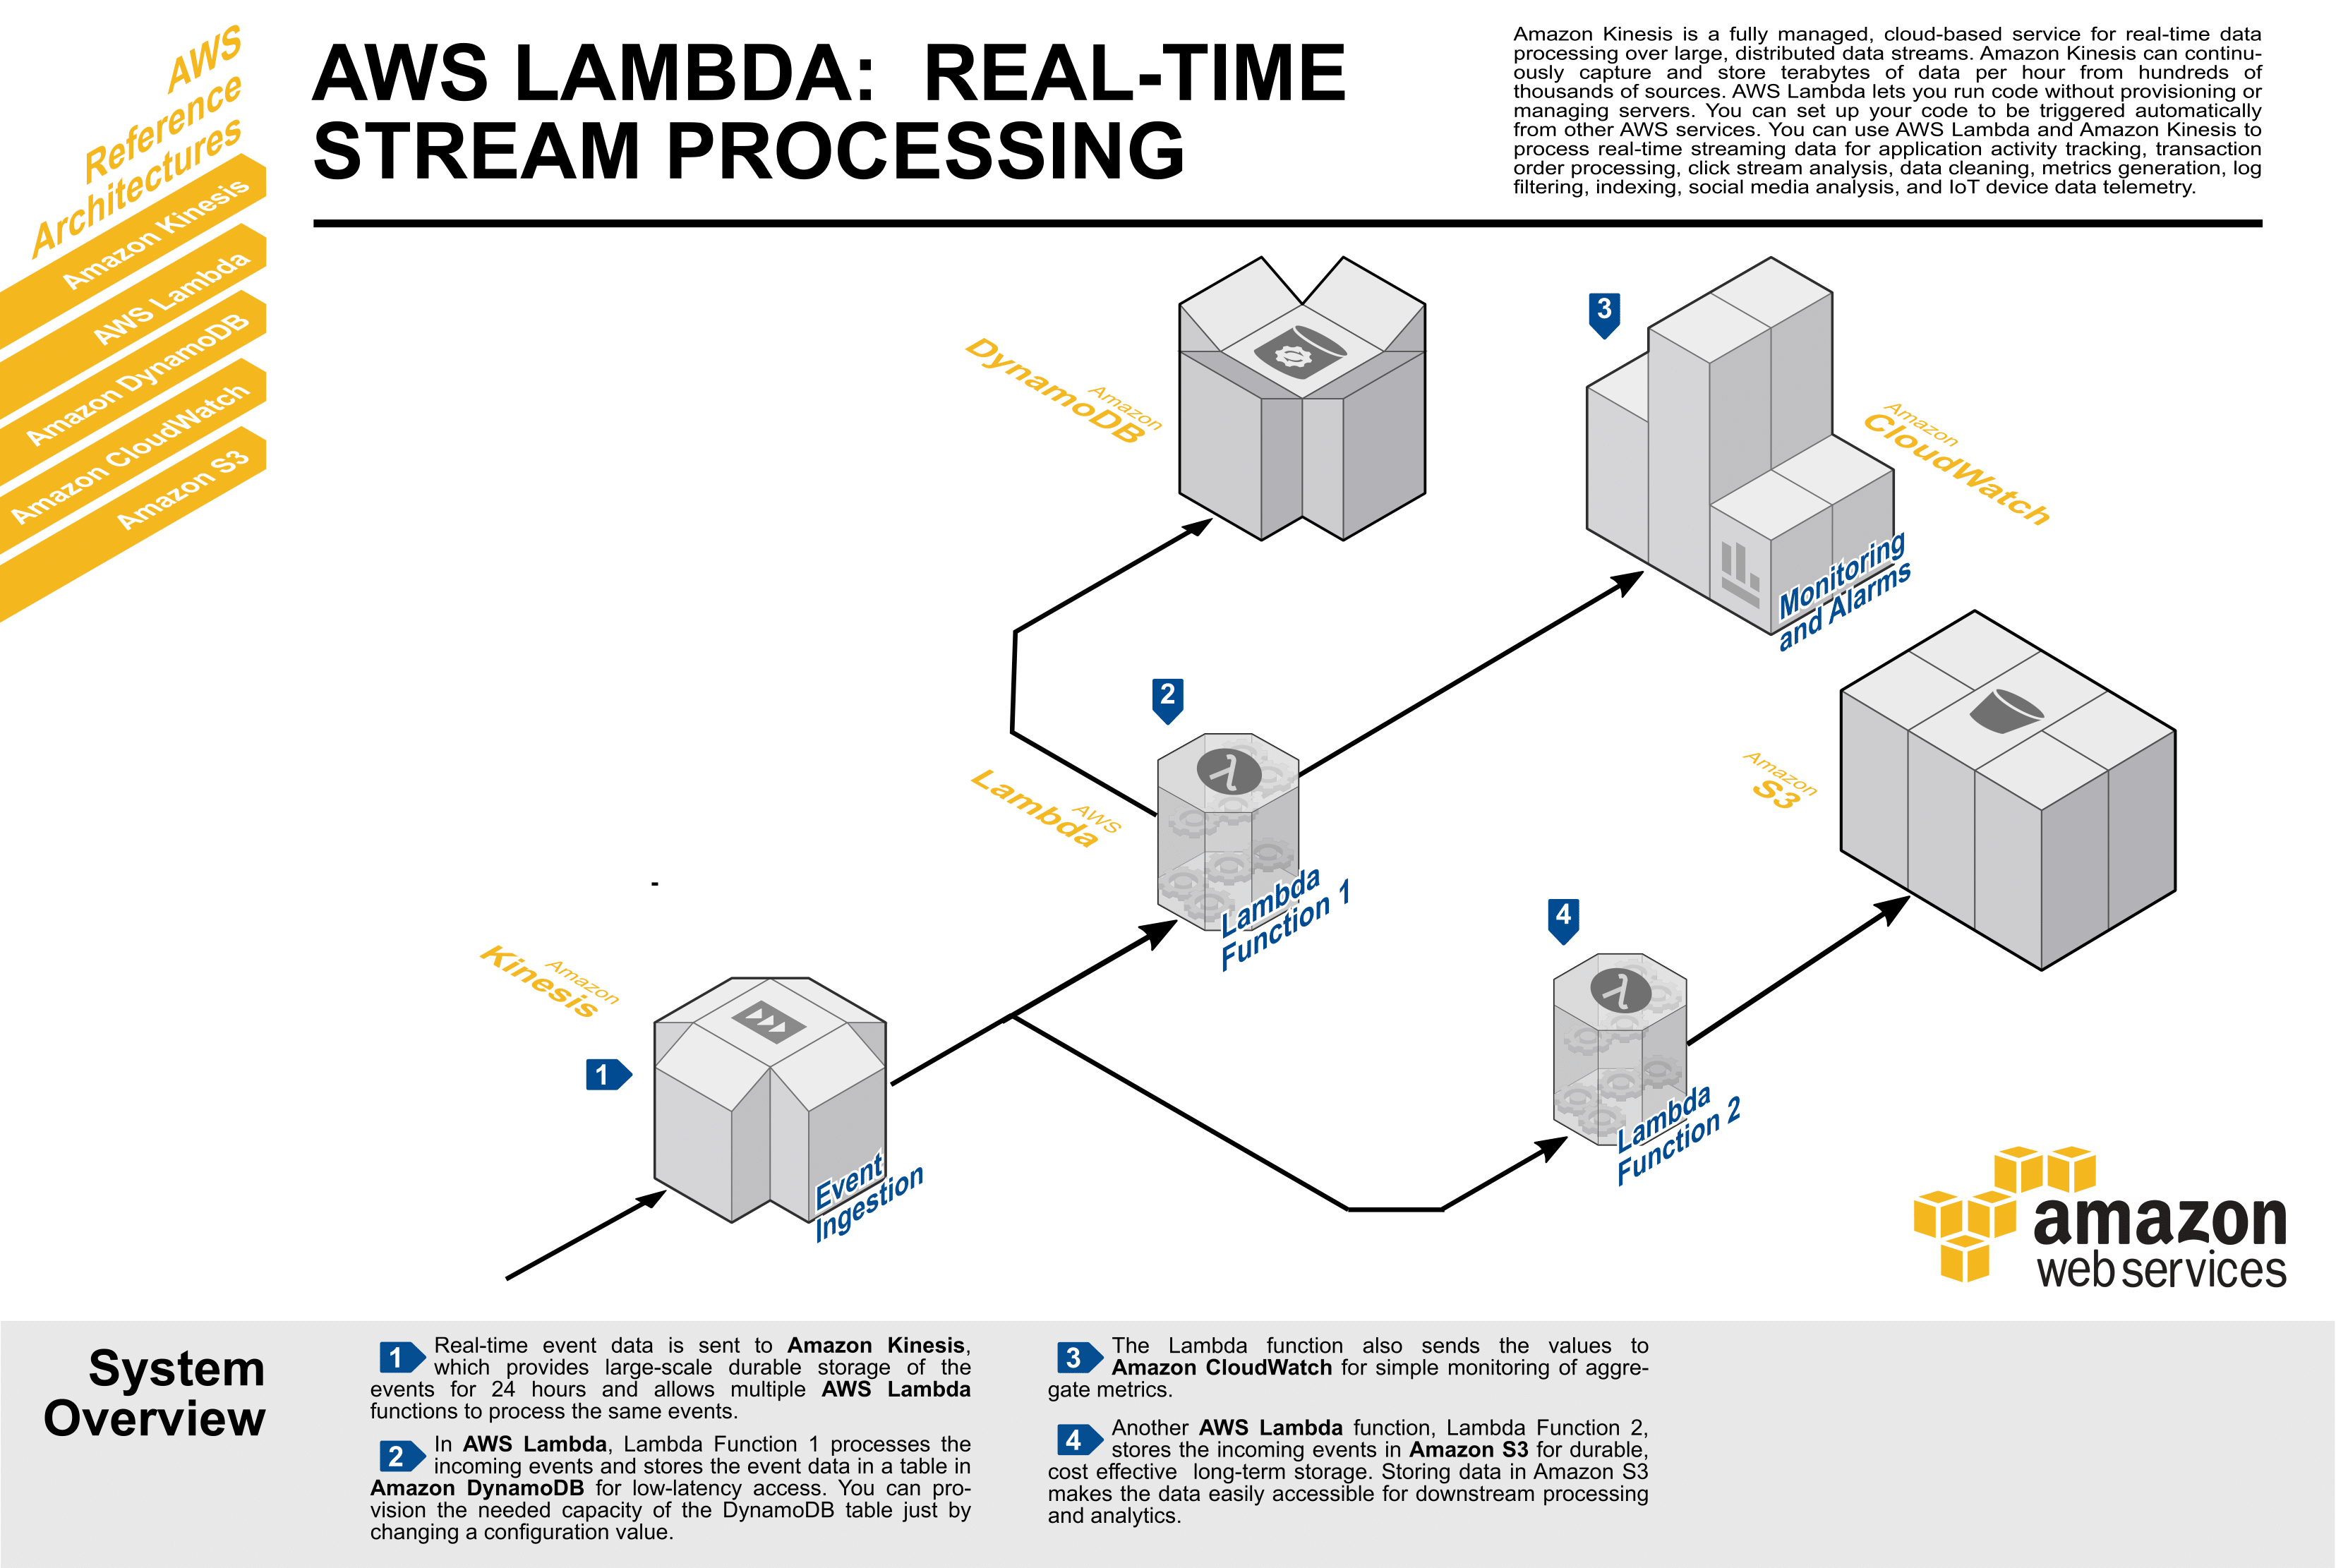
\includegraphics[width=0.45\textwidth]{images/lambda-refarch-streamprocessing.png}}
	\caption{Researched AWS Reference Architecture}%
	\label{fig:aws-refarch}%
\end{figure}

All presented and more reference architectures can be found at https://github.com/awslabs. The following list includes the links to the discussed architectures:

\begin{itemize}
\tightlist
\item
  https://github.com/awslabs
\item
  https://github.com/awslabs/lambda-refarch-iotbackend
\item
  https://github.com/awslabs/lambda-refarch-streamprocessing
\item
  https://github.com/awslabs/ecs-refarch-batch-processing
\end{itemize}

\subsection{Evolution of the architecture}\label{evolution-of-the-architecture}

As the project evolved and the understanding of the domain increased the
architecture evolved as well. It is the nature of an agile project to
evolve over time when the product owners add features to the system.
This section will present an overview of the evolution of the
architecture and the changes done over time.

The changes in architecture are depicted in figure \ref{fig:architecture_1}.

\begin{figure}
		\subfigure[Initial Architecture]{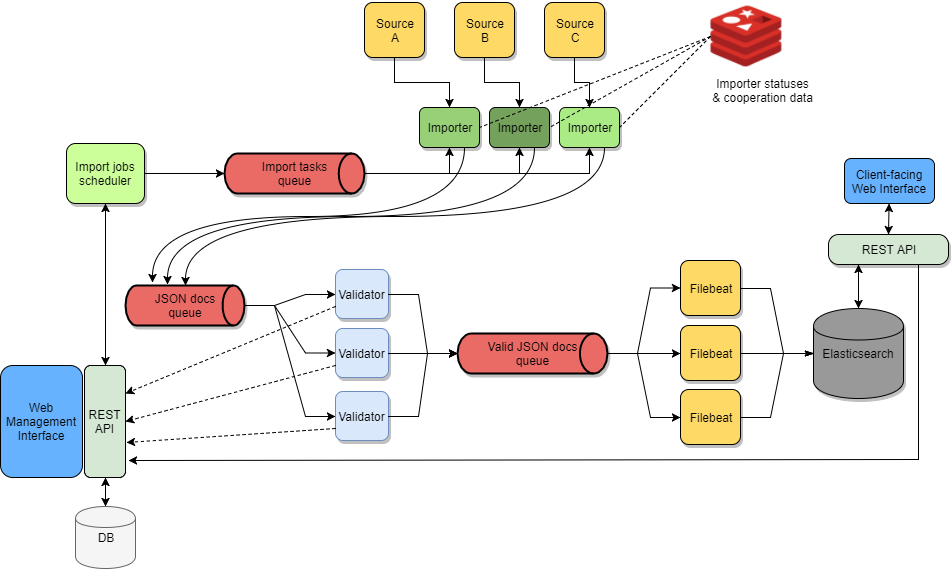
\includegraphics[width=0.45\textwidth]{images/170713_architecture_1.png}} 
		\subfigure[Final Architecture]{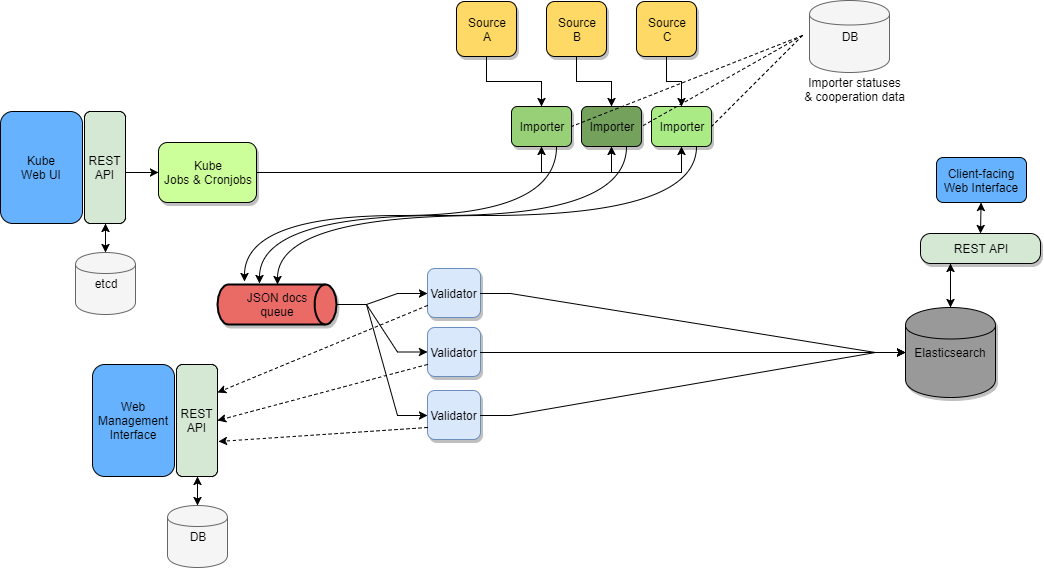
\includegraphics[width=0.45\textwidth]{images/170713_architecture4.png}}
	\caption{Evolution of Architecture}
	\label{fig:evol_architecture}
\end{figure}

Basically, the architecture was
update at two places. First, the scheduling logic was exchanged. In the
final architecture, we rely on Kubernetes and cron jobs to schedule the
importing tasks. We decided for Kubernetes to administrate the
underlying infrastructure thus it was feasible to use it for scheduling
as well. The underlying infrastructure will be discussed in more detail
in chapter \ref{sec:infrastructure}, but since the placement and deployment
of components is done with Kubernetes we decided to use it to schedule
the importers.

Additionally, filebeat and one messaging queue got removed. To reduce
latency the latency of the system, the validator and filebeat were
merged into one component, the consumer. This changed made the messaging
queue in between those components obsolete. At this point we coupled
functionality and added dependency but the increased performance made up
for it.

Summarizing, we exchanged one building block with a better alternative
and shortened our pipeline in order to increase throughput.

\subsection{Discussion}\label{discussion}

Summarizing, we designed a fault-tolerant, highly scalable and available
architecture based on the microservice design. The architecture is
formed of several independent and loosely coupled services that interact
through technology-agnostic interfaces. By doing so, we could use
different technologies for every component and develop each building
block independently.

On the flip side, we created a highly complex architecture consisting of
several technologies and services, which makes it hard to be understood
by a single person. Furthermore, the deployment and operation of the
system has to be automated otherwise an administrator might reach his
limit quickly. We offer scripts to deploy the system onto AWS, but this
can be applied to every other cloud provider or a private cloud with
minor changes.

\subsection{Future}\label{future}

No system is perfect hence, in this section we propose some possible
future updates that might improve the proposed solution. The major value
of the designed system is the possibility to retrieve open environmental
data through a uniform interface. In other words, the query performance
of our database solution is of main concern. A possibility to increase
query performance for complex requests might be the implementation of an
interaction between the public API, exposed to the user, and the Data
Source Metadata Management System. By doing so, the API could learn
which indexes include the data to answer a specific query in contrast to
answering the query in a naive way and leaving the optimization solely.

A different approach to improve the system might be the introduction of
a serverless component. Though, this proposal only applies to a solution
deployed on a public or hybrid cloud that offers such services. Such a
serverless service might replace a functionality or module of an
importing task. For example, one could use it to for unit conversion. On
the other hand, it might be necessary to perform benchmarks and evaluate
the added value through a serverless component. Since we release
resources immediately after a job finishes, it is hard to tell if it
really is more cost efficient without proper testing.
